\chapter{Data Visualization}

The final dataset has 189297 rows × 15 columns. The columns are as follows: 
\begin{table}[h!]
    \centering
    \begin{tabular}{lllll} % 5 columns per row
    \toprule
    \textbf{danceability} & \textbf{energy} & \textbf{key} & \textbf{loudness} & \textbf{mode} \\
    \textbf{speechiness} & \textbf{acousticness} & \textbf{instrumentalness} & \textbf{liveness} & \textbf{valence} \\
    \textbf{tempo} & \textbf{duration\_ms} & \textbf{time\_signature} & \textbf{region} & \textbf{popular} \\
    \bottomrule
    \end{tabular}
    \caption{Column names in the dataset}
\end{table}

By visualizing and exploring the final dataset, we can underline the differeces with the raw dataset. This shows that the preprocessing phase was fundamental to obtain a clean dataset.

\begin{verbatim}
    # Display the first few rows of the dataset
    df.head()
    
    # Display basic information about the dataset
    df.info()
    \end{verbatim}
    
    \begin{figure}[h]
        \centering
        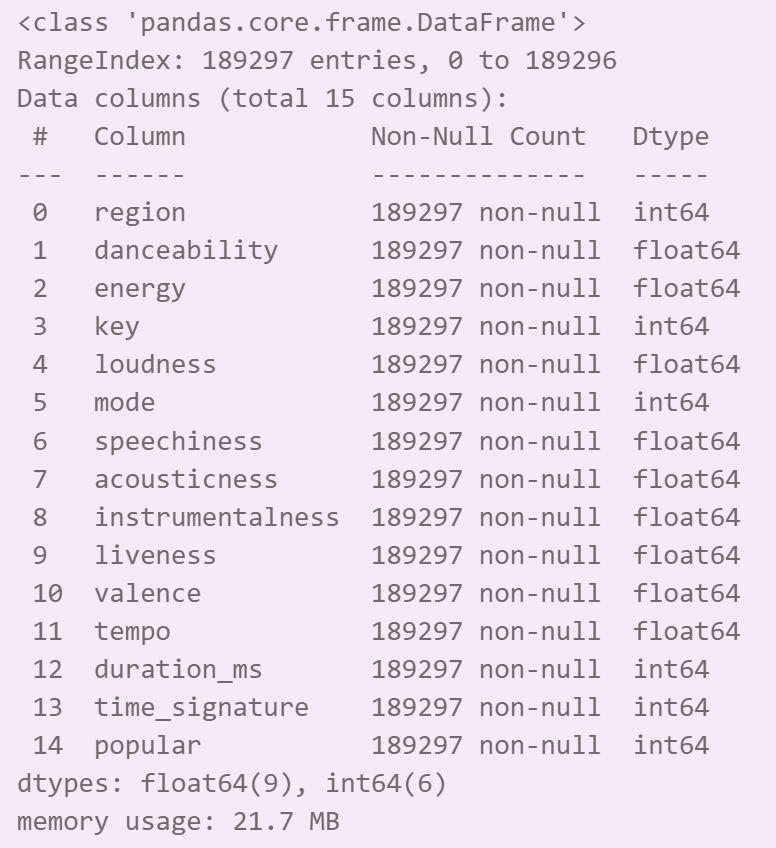
\includegraphics[width=0.5\textwidth]{media/info_cleaned.png} 
        \caption{Basic information.}
        \label{df.info()}
    \end{figure}

    One of the first thing to notice is how the memory usage has been reduced significantly. This is due to the removal of columns that were not useful for the analysis. In fact, the number of columns has been reduced from 26 to 15.
    
    \newpage
    \begin{verbatim}
    # Summary statistics of the dataset
    df.describe()
    \end{verbatim}
    
    
    \begin{figure}[h]
        \centering
        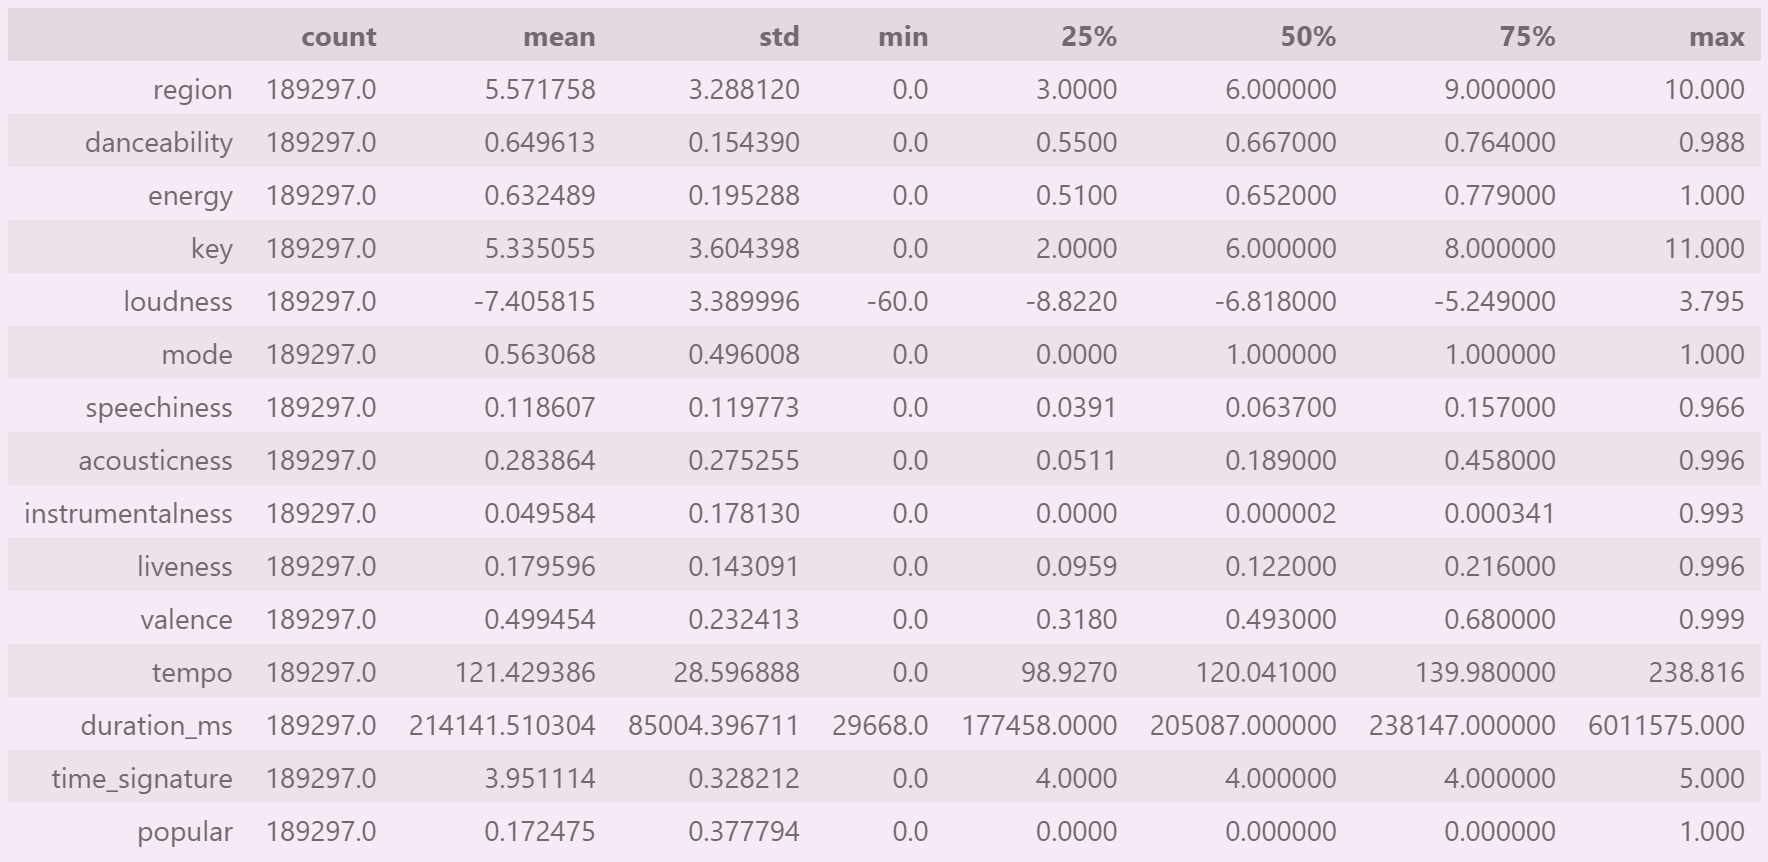
\includegraphics[width=1.1\textwidth]{media/describe_cleaned.png} 
        \caption{Summary statistics of the dataset.}
        \label{df.describe()}
    \end{figure}

The popular songs represent about the 20\% of the dataset.

    \begin{figure}[h]
        \centering
        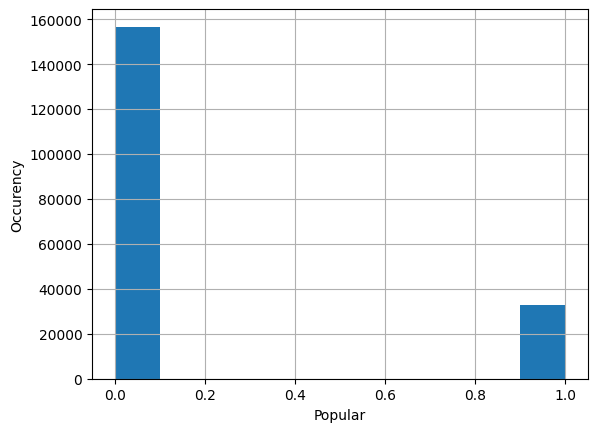
\includegraphics[width=0.5\textwidth]{media/popular_dist_cleaned.png} 
        \caption{Distribution of popular songs.}
        \label{popular_songs}
    \end{figure}

\newpage

Each audio feature is distributed in this way: 

\begin{figure}[h]
    \centering
    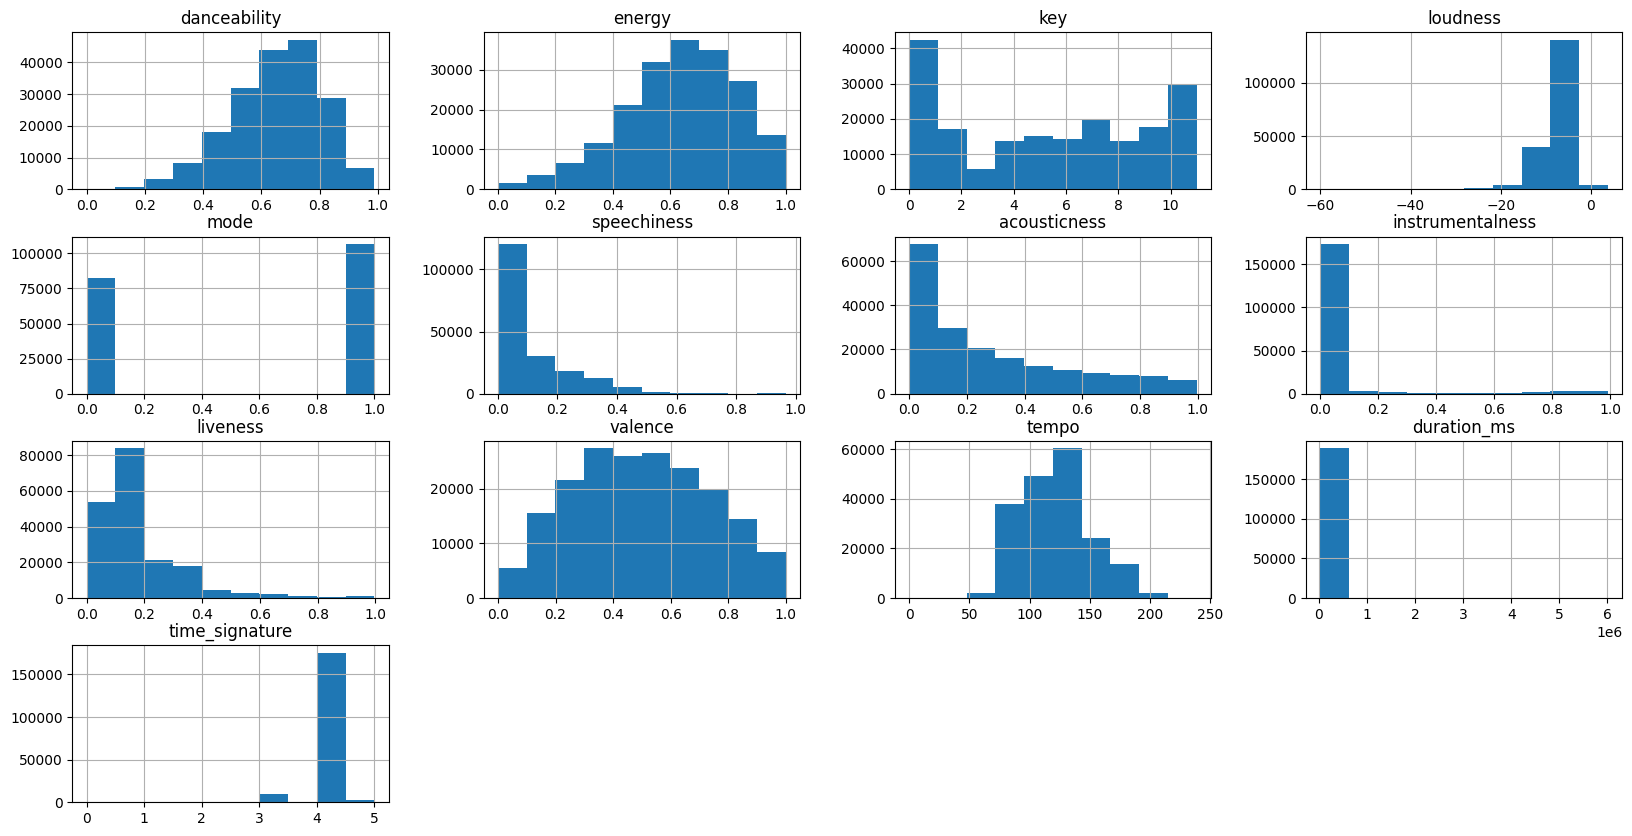
\includegraphics[width=0.9\textwidth]{media/feature_dist_cleaned.png} 
    \caption{Distribution of audio features.}
    \label{distribution}
\end{figure}

This is the boxplot of the audio features:

\begin{figure}[h]
    \centering
    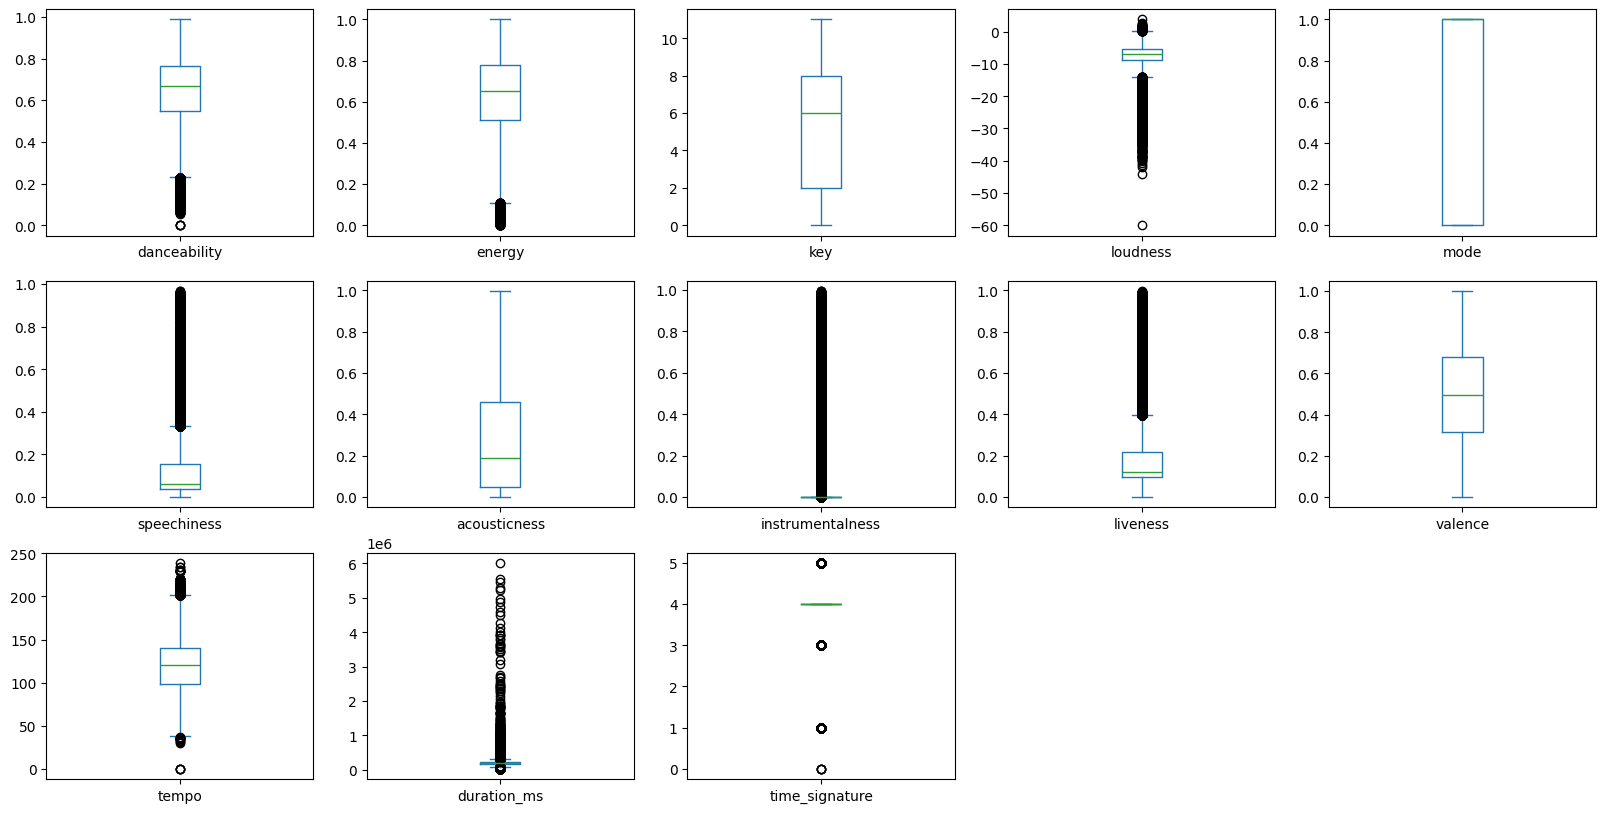
\includegraphics[width=0.9\textwidth]{media/boxplot_cleaned.png} 
    \caption{Boxplot of audio features.}
    \label{boxplot}
\end{figure}


Many features have outliers (especially loudness, instrumentalness, speechiness, and duration\_ms), which means they have songs that are very different from the "average" in terms of these attributes.
Features like mode and time\_signature have almost no variation, thus they may not be useful for predicting the target variable (popularity).


\newpage

This is the heatmap of the correlation matrix:

\begin{figure}[h]
    \centering
    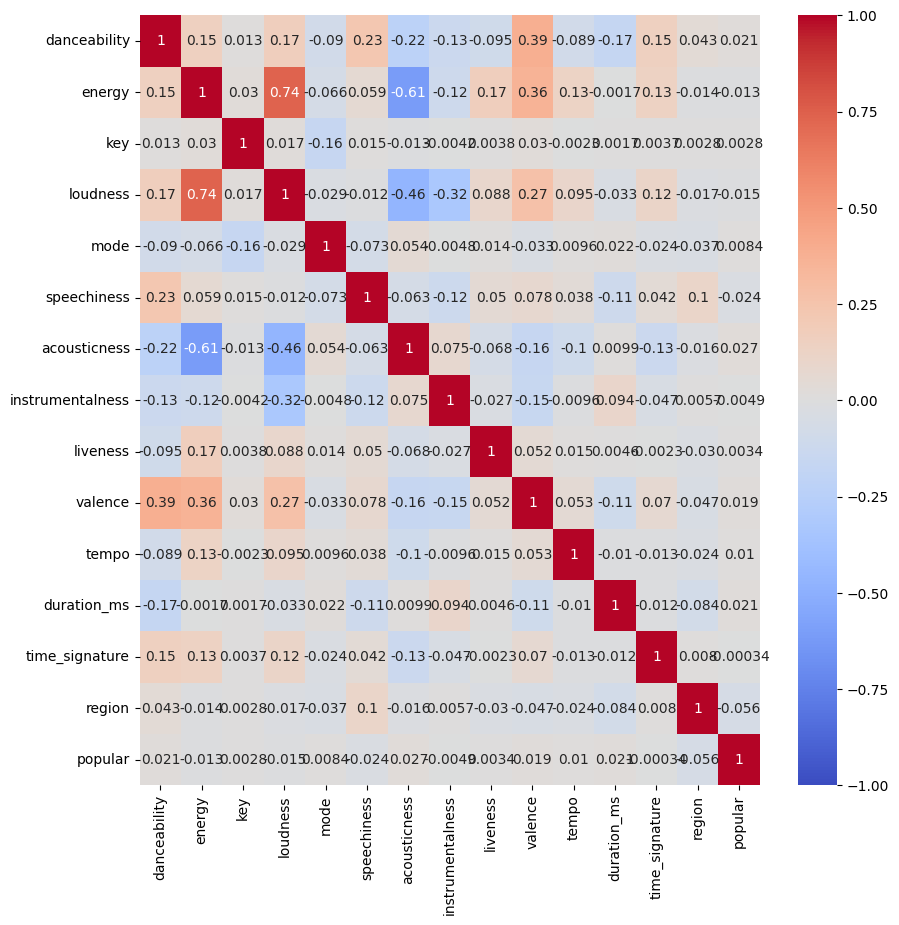
\includegraphics[width=0.9\textwidth]{media/heatmap_cleaned.png} 
    \caption{Heatmap of the correlation matrix.}
    \label{correlation}
\end{figure}

The heatmap shows that the audio features have a mix of positive and negative correlations with each other. The most notable correlations are:
\begin{itemize}
    \item 
    Energy and Loudness: strong positive correlation (0.74). Loud songs tend to also have high energy, which makes sense musically.
    \item Energy and Acousticness: strong negative correlation  (-0.61). Acoustic songs tend to have lower energy levels, which aligns with expectations as acoustic songs are often more mellow.
\end{itemize}


This also shows us that no single feature stands out as highly predictive of song popularity based on these correlations, which suggests that popularity might be determined by a complex interaction of features rather than individual attributes. 



\newpage

We can also visualize the popularity of each feature in the different regions:

\begin{figure}[h]
    \centering
    \begin{minipage}{0.45\textwidth}
        \centering
        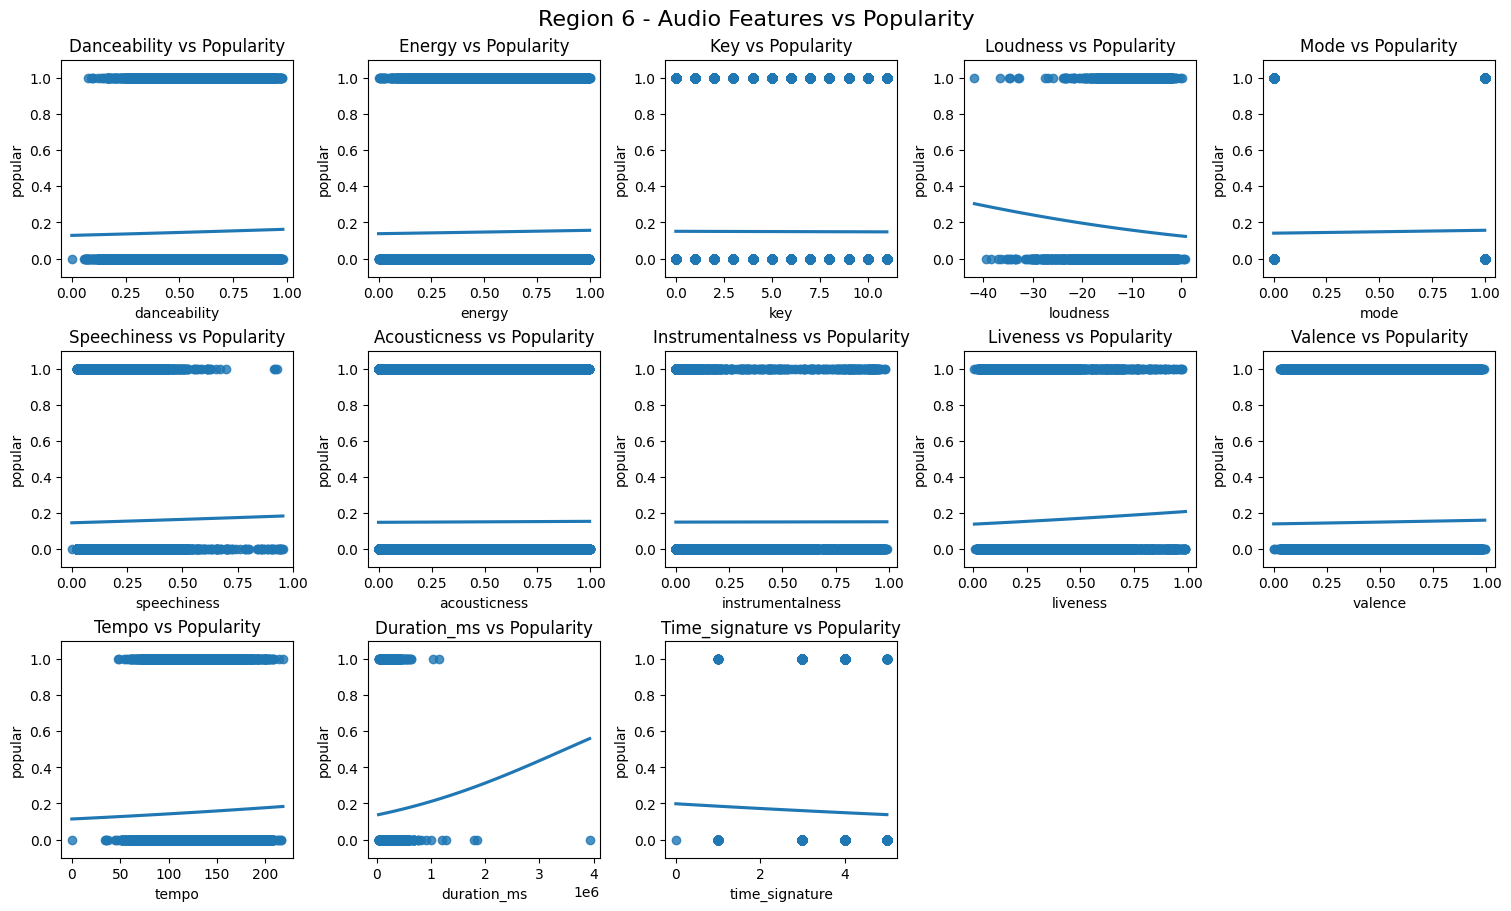
\includegraphics[width=\linewidth]{media/region6_cleaned.png}
        \caption{Popularity in Northern Europe}
        \label{northern_europe}
    \end{minipage}%
    \hspace{0.05\textwidth}
    \begin{minipage}{0.45\textwidth}
        \centering
        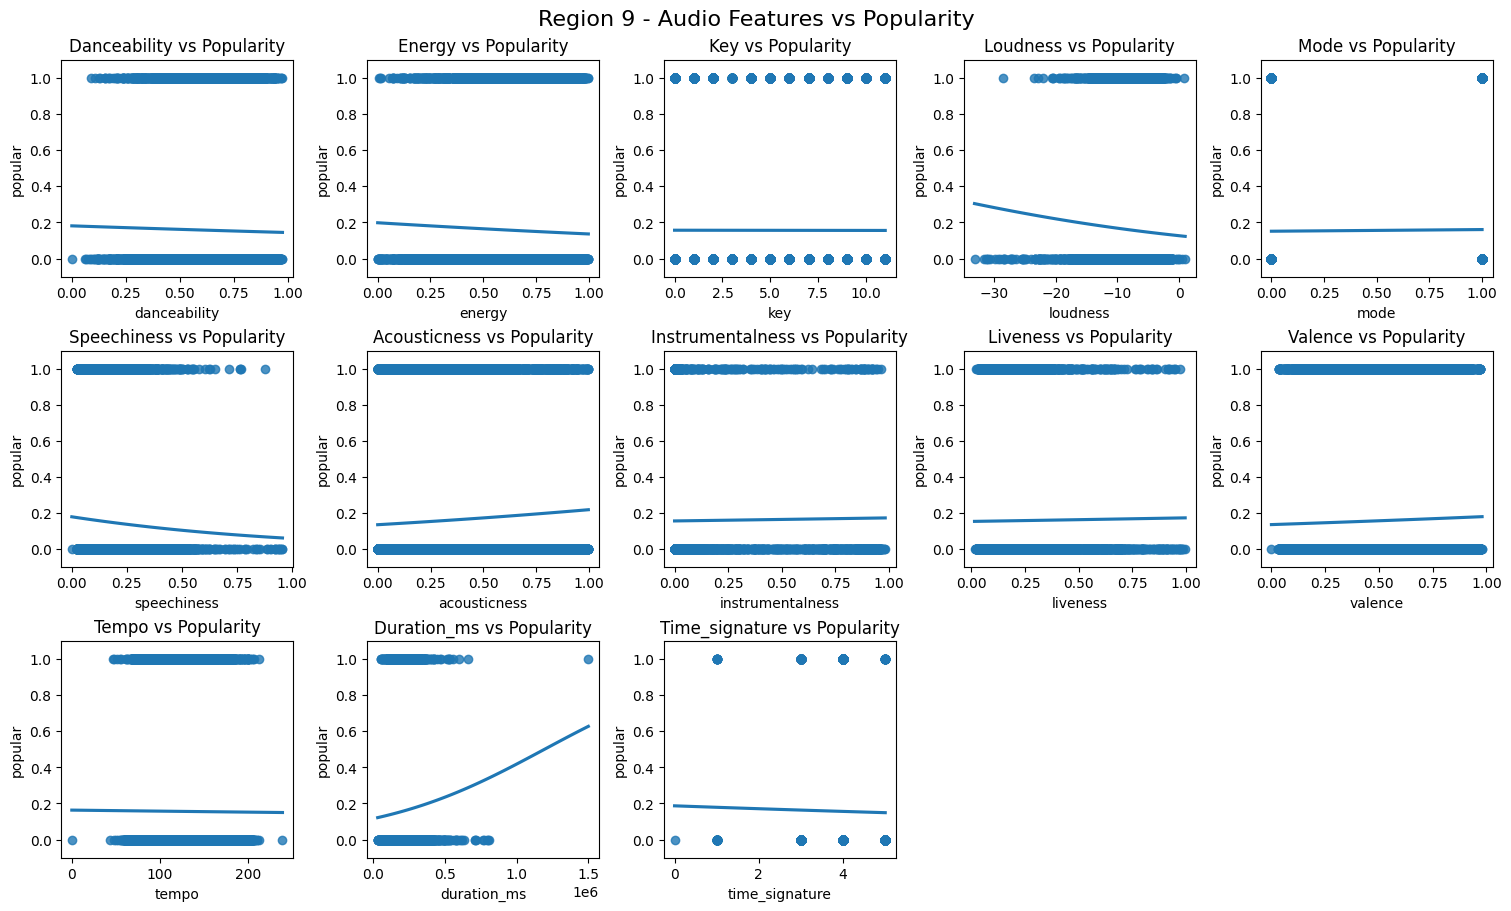
\includegraphics[width=\linewidth]{media/region9_cleaned.png}
        \caption{Popularity in Southern Europe}
        \label{southern_europe}
    \end{minipage}
    
    \vspace{0.05\textwidth}
    
    \begin{minipage}{0.45\textwidth}
        \centering
        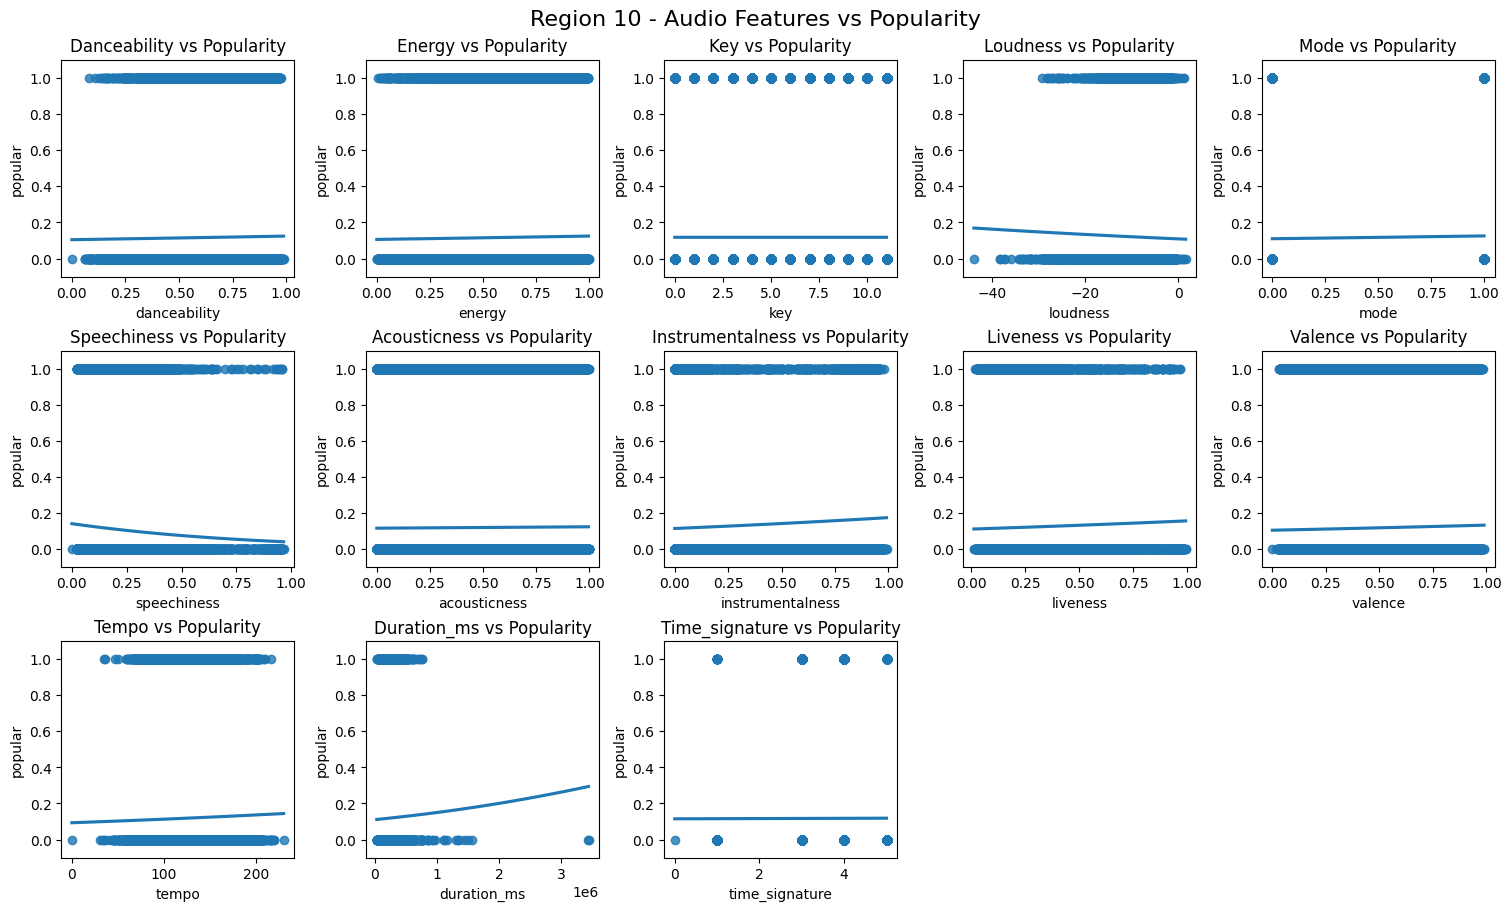
\includegraphics[width=\linewidth]{media/region10_cleaned.png}
        \caption{Popularity in Western Europe}
        \label{western_europe}
    \end{minipage}%
    \hspace{0.05\textwidth}
    \begin{minipage}{0.45\textwidth}
        \centering
        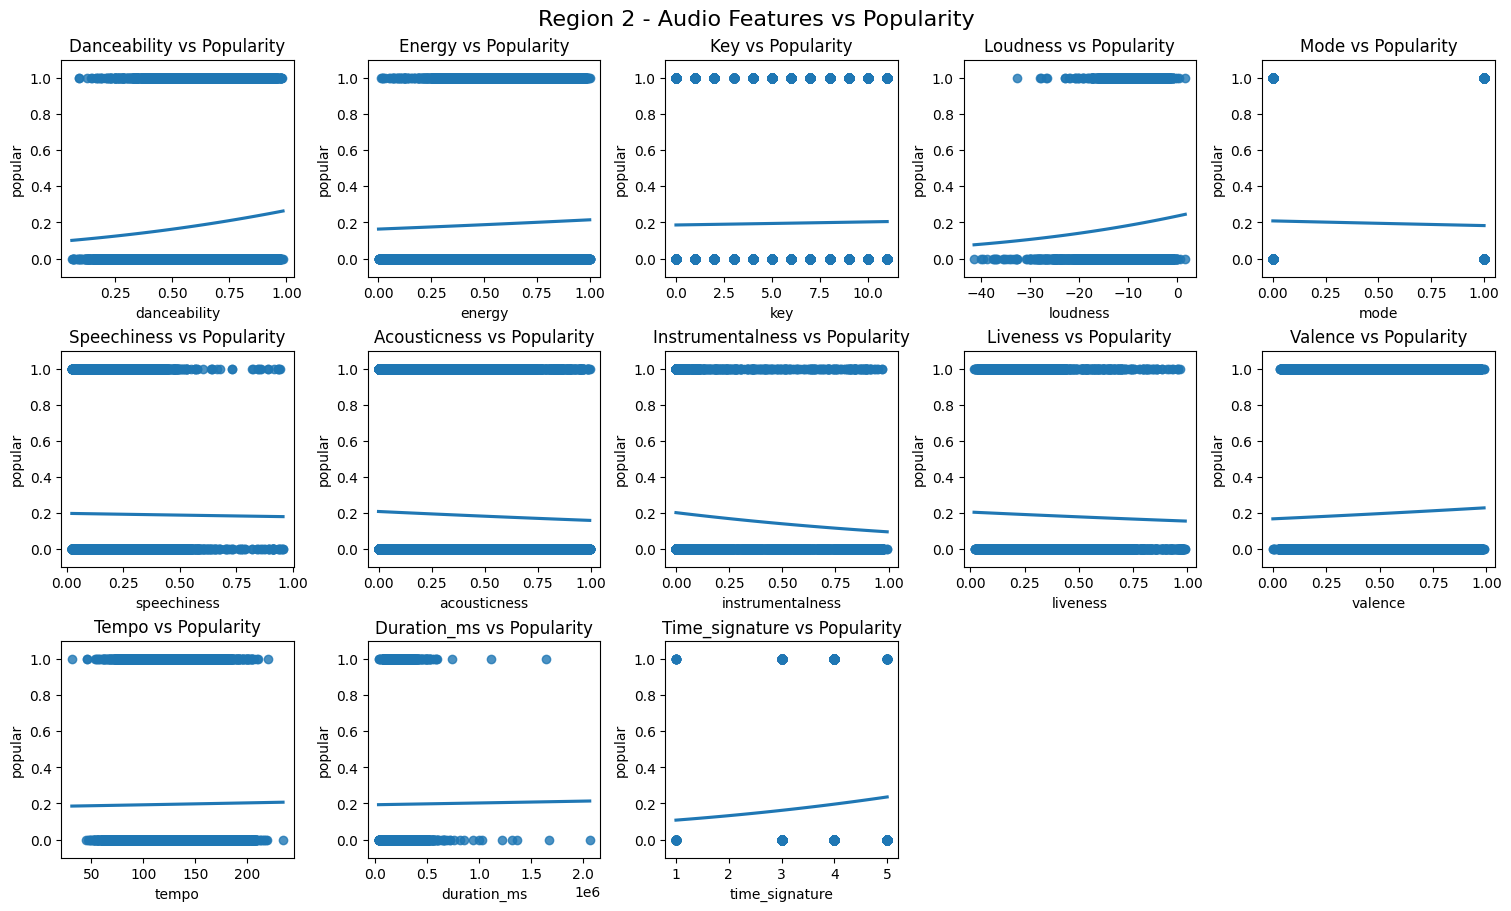
\includegraphics[width=\linewidth]{media/region2_cleaned.png}
        \caption{Popularity in Eastern Europe}
        \label{eastern_europe}
    \end{minipage}
    
    \vspace{0.05\textwidth}
    
    \begin{minipage}{0.45\textwidth}
        \centering
        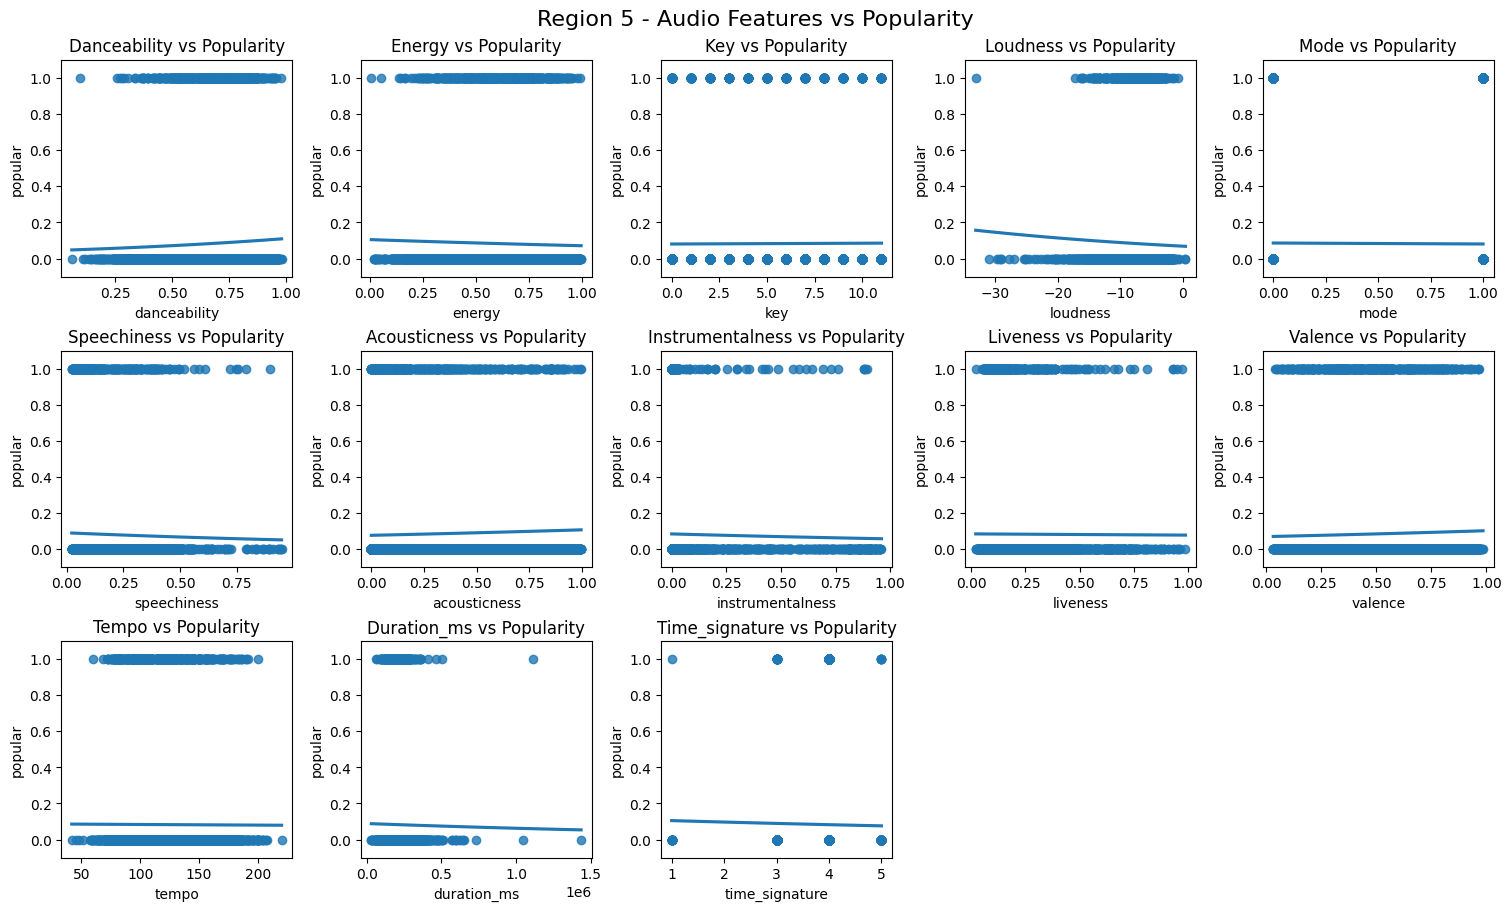
\includegraphics[width=\linewidth]{media/region5_cleaned.png}
        \caption{Popularity in North America}
        \label{north_america}
    \end{minipage}%
    \hspace{0.05\textwidth}
    \begin{minipage}{0.45\textwidth}
        \centering
        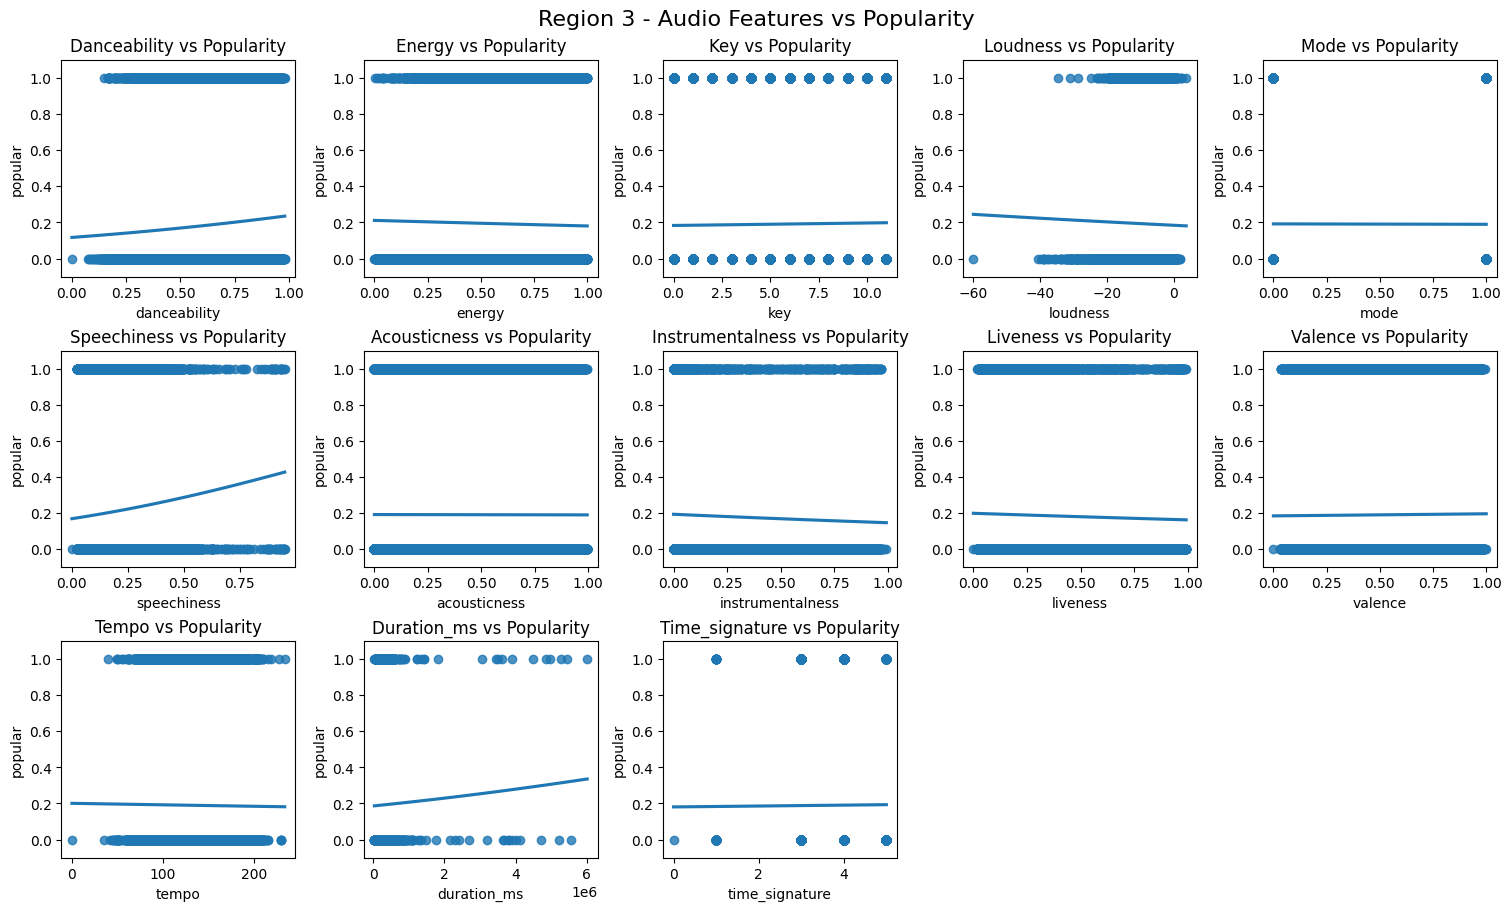
\includegraphics[width=\linewidth]{media/region3_cleaned.png}
        \caption{Popularity in Latin America}
        \label{latin_america}
    \end{minipage}
\end{figure}

\clearpage % Force new page after 6 figures

\begin{figure}[h]
    \centering
    \begin{minipage}{0.45\textwidth}
        \centering
        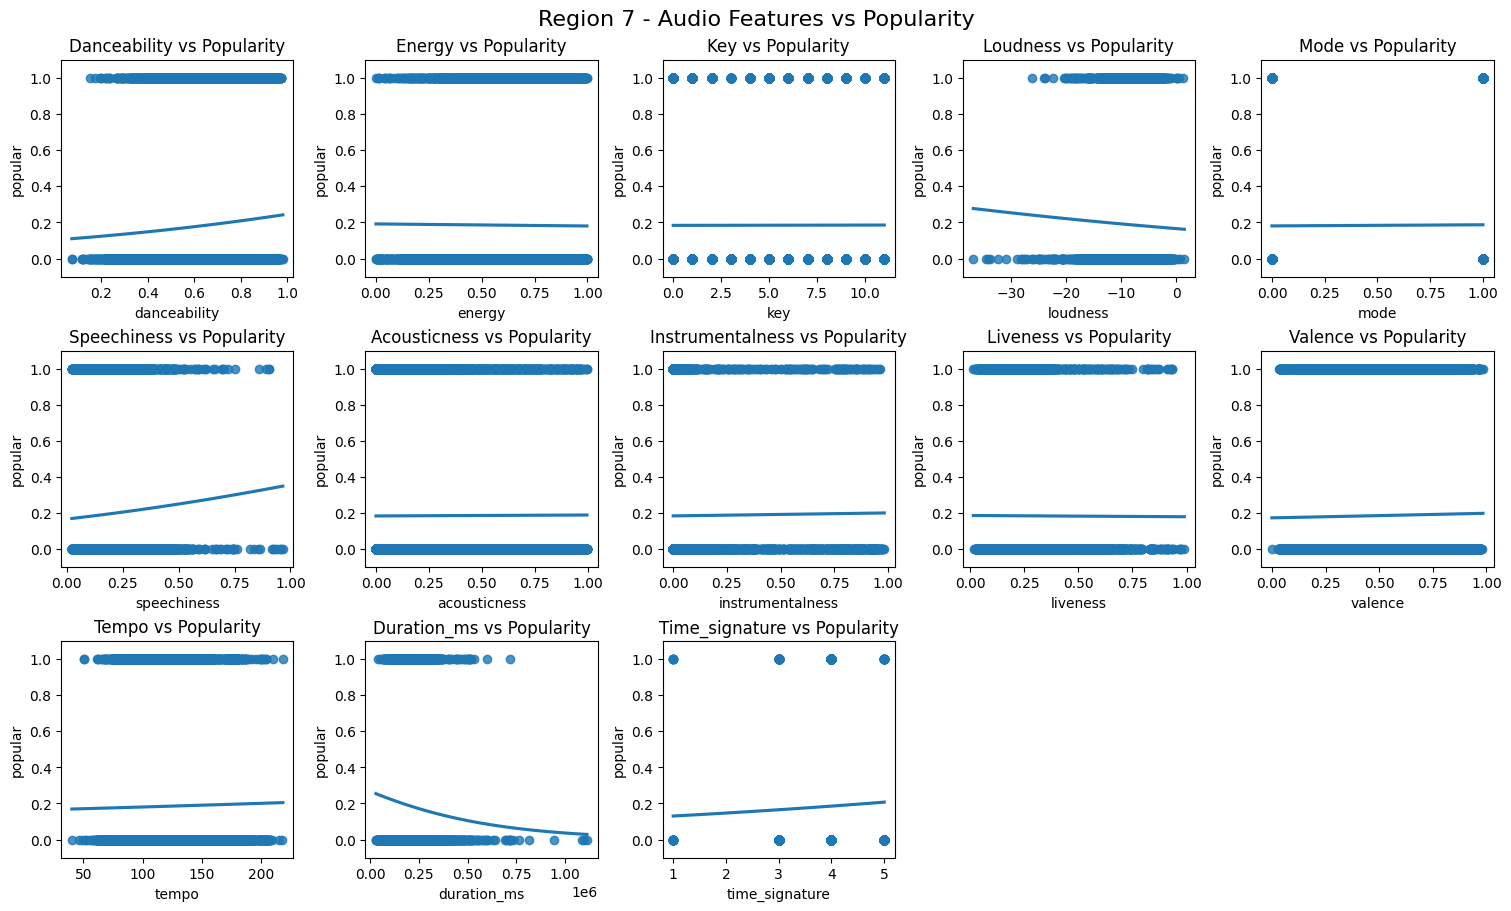
\includegraphics[width=\linewidth]{media/region7_cleaned.png}
        \caption{Popularity in Oceania}
        \label{oceania}
    \end{minipage}%
    \hspace{0.05\textwidth}
    \begin{minipage}{0.45\textwidth}
        \centering
        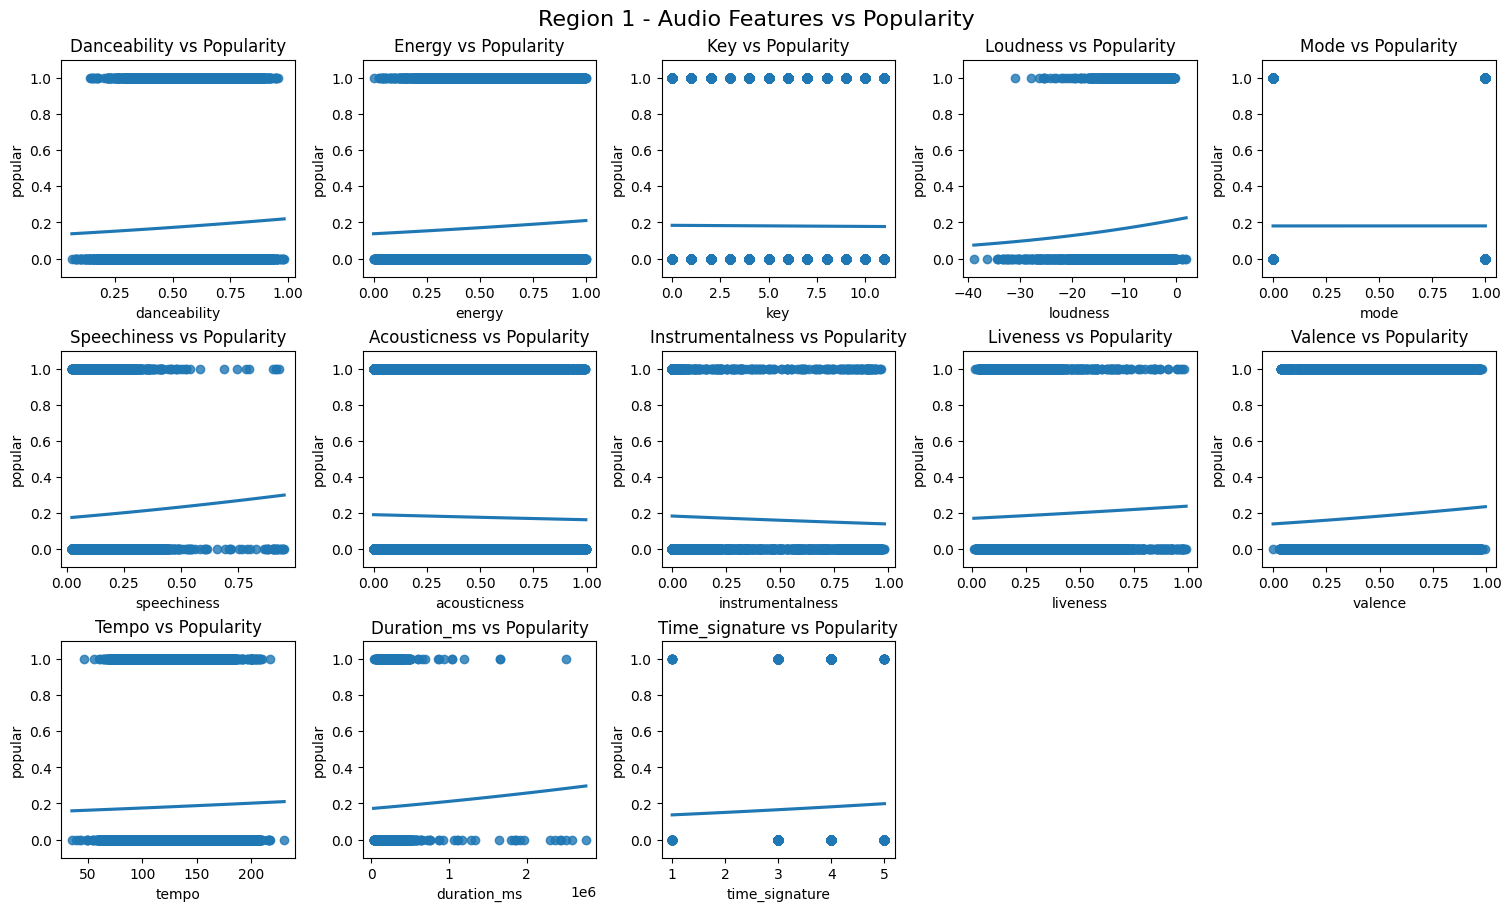
\includegraphics[width=\linewidth]{media/region1_cleaned.png}
        \caption{Popularity in East Asia}
        \label{east_asia}
    \end{minipage}
    
    \vspace{0.05\textwidth}
    
    \begin{minipage}{0.45\textwidth}
        \centering
        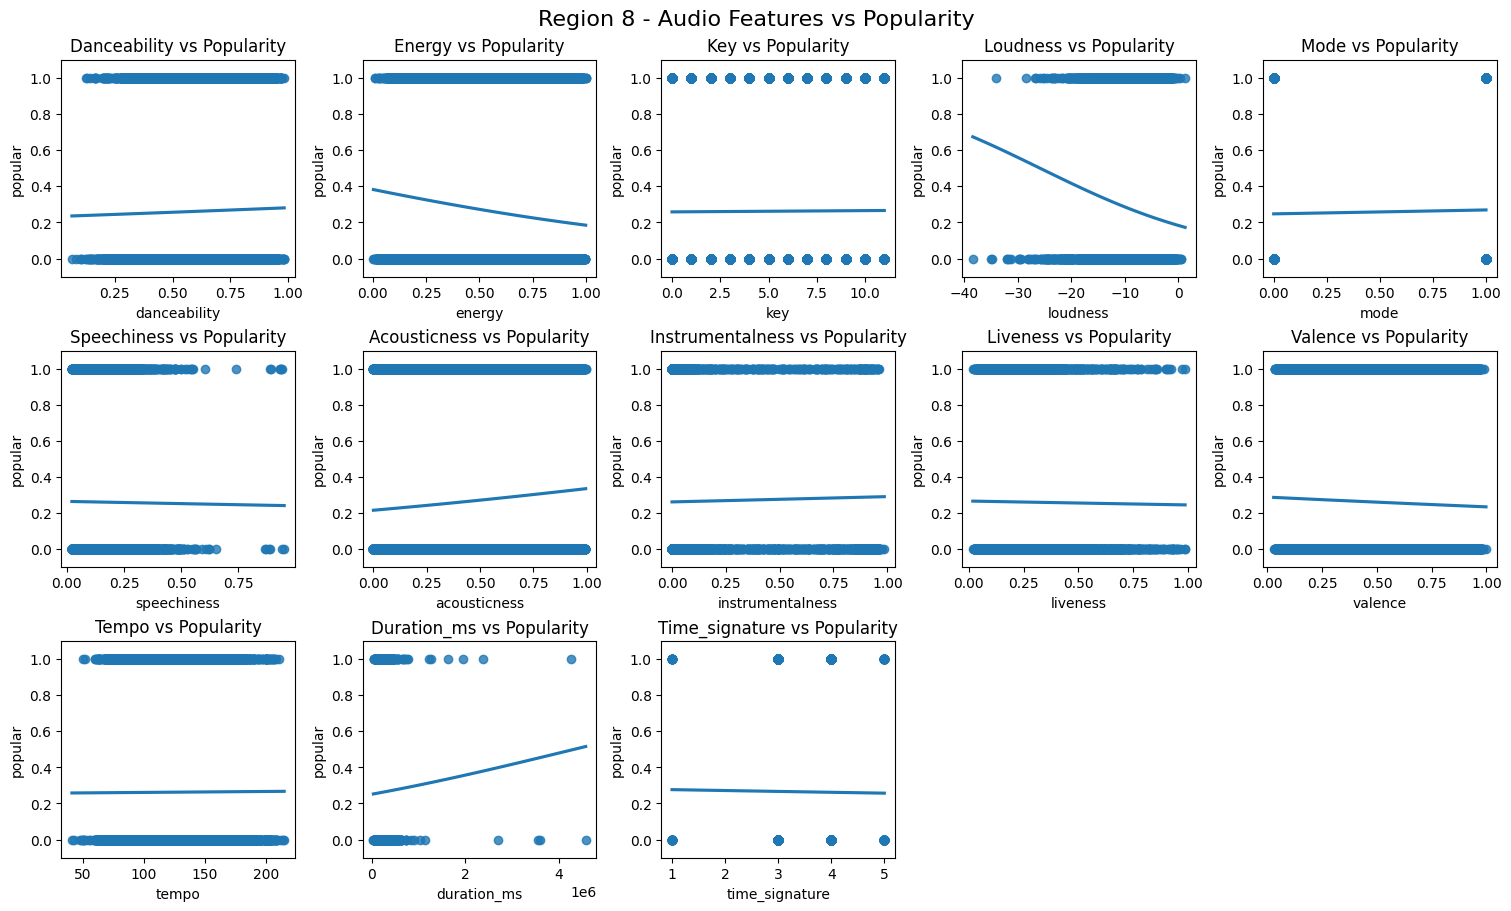
\includegraphics[width=\linewidth]{media/region8_cleaned.png}
        \caption{Popularity in South Asia}
        \label{south_asia}
    \end{minipage}%
    \hspace{0.05\textwidth}
    \begin{minipage}{0.45\textwidth}
        \centering
        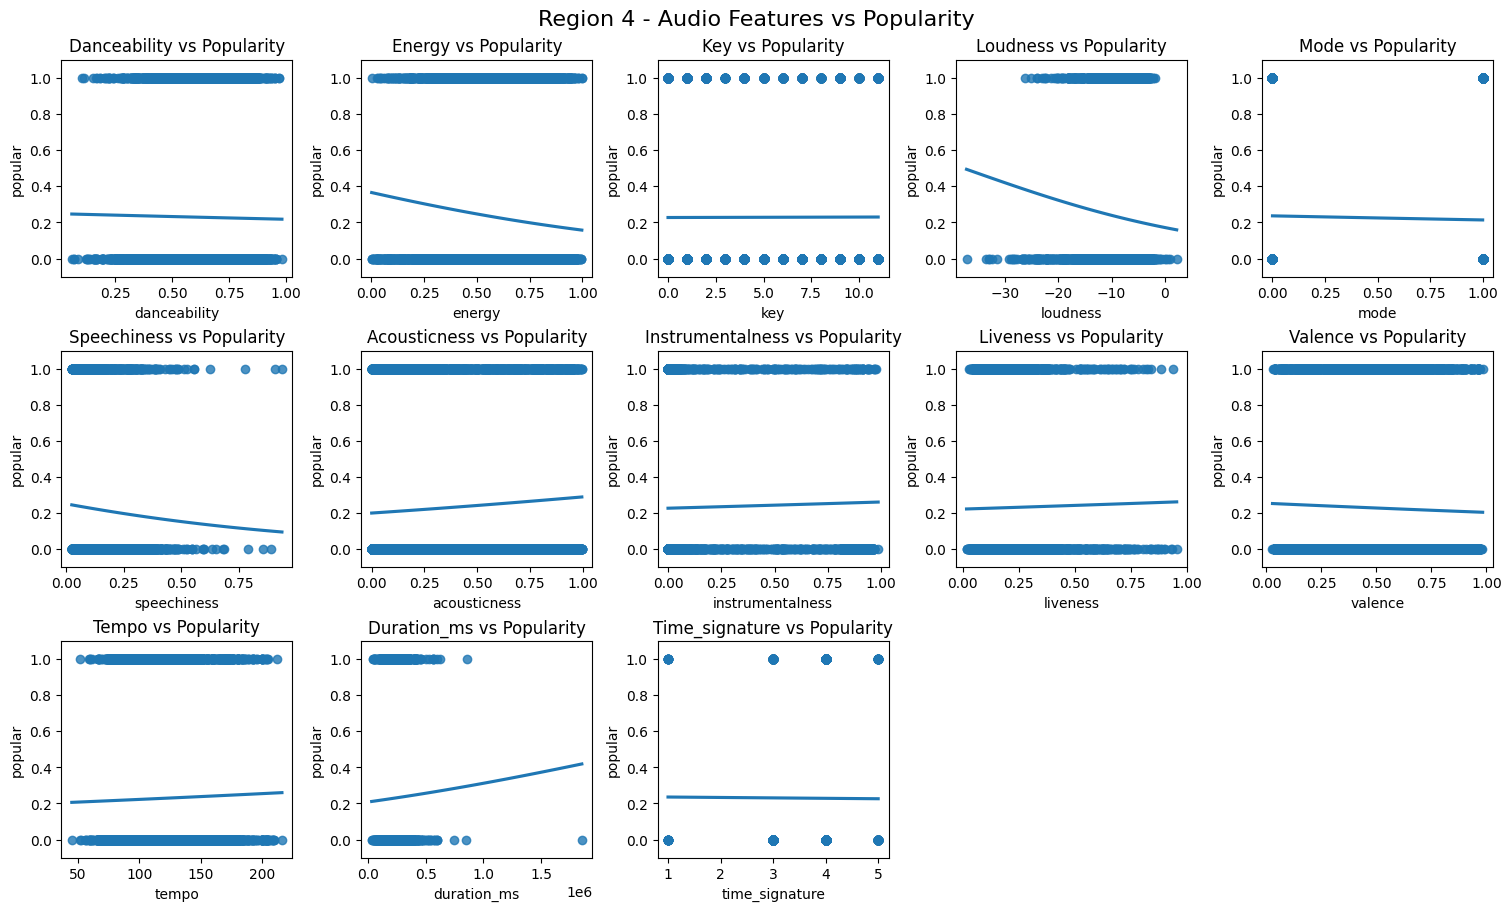
\includegraphics[width=\linewidth]{media/region4_cleaned.png}
        \caption{Popularity in the Middle East}
        \label{middle_east}
    \end{minipage}
\end{figure}

\begin{figure}[h]
    \centering
    \begin{minipage}{0.45\textwidth}
        \centering
        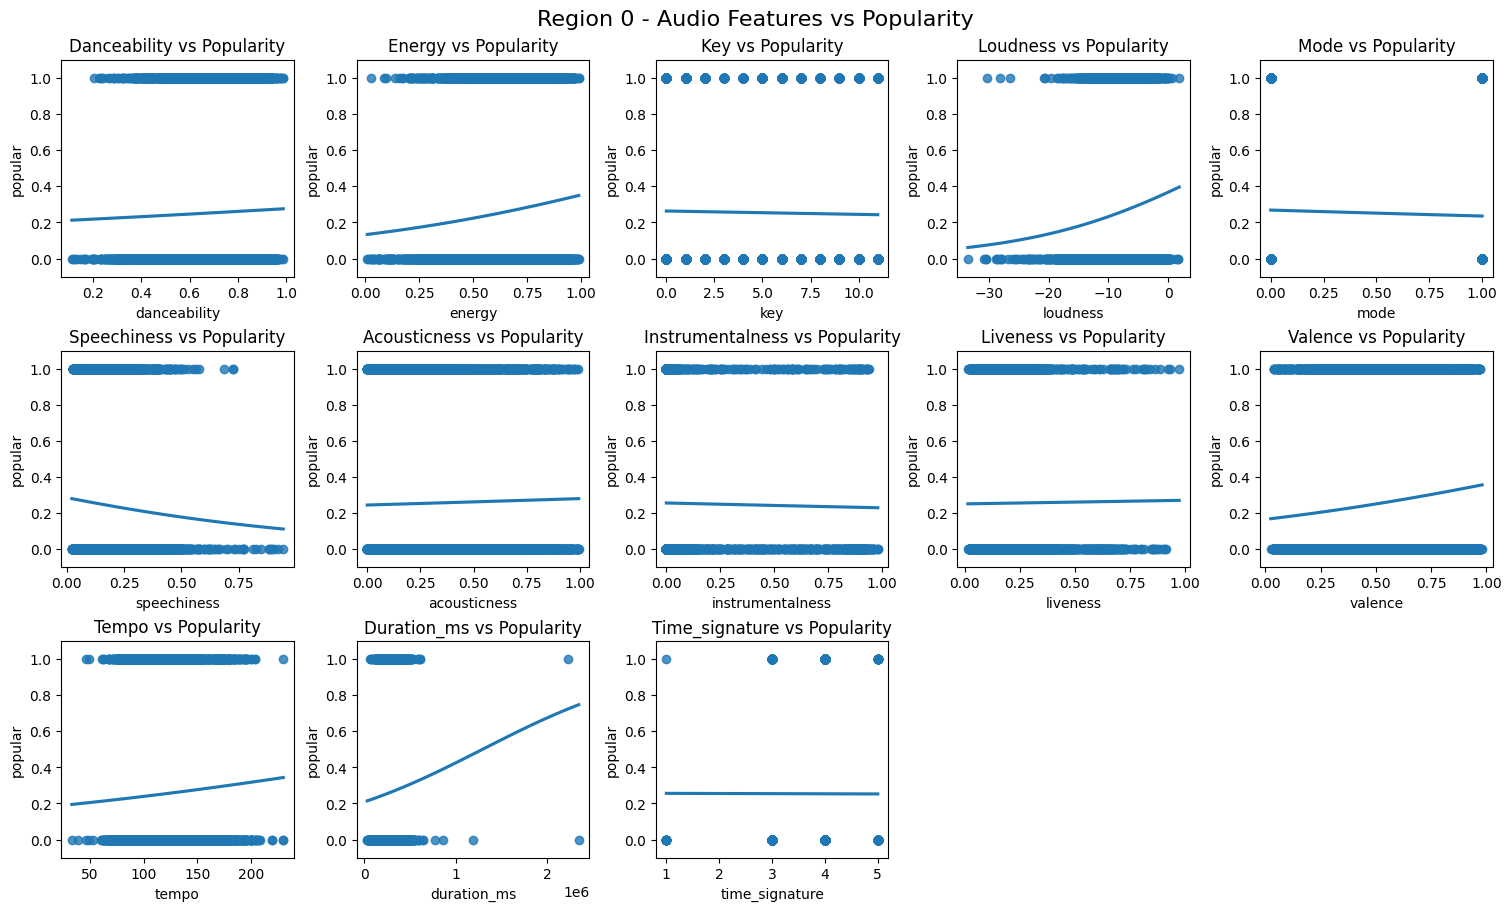
\includegraphics[width=\linewidth]{media/region0_cleaned.png}
        \caption{Popularity in Africa}
        \label{africa}
    \end{minipage}
\end{figure}


This allows us to understand what features make a song popular or not in the different regions.

\begin{itemize}
    \item \textbf{Northern Europe}: energy and danceability
    \item \textbf{Southern Europe}: acousticness and valence
    \item \textbf{Eastern Europe}: danceability
    \item \textbf{North America}: danceability and acousticness
    \item \textbf{Latin America}: speechiness and danceability
    \item \textbf{Oceania}: danceability and energy
    \item \textbf{East Asia}: valence
    \item \textbf{South Asia}: danceability and acousticness
    \item \textbf{Middle East}: danceability
    \item \textbf{Africa}: loudness, valence, acousticness, duration and tempo
    
\end{itemize}
   

\begin{figure}[H]
    \centering
    \begin{minipage}{0.45\textwidth}
        \centering
        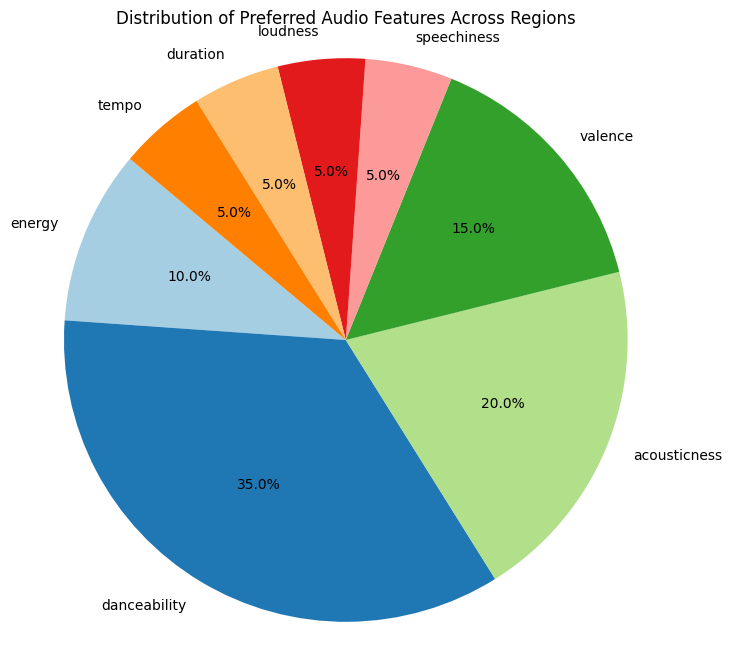
\includegraphics[width=\textwidth]{media/features_preferences.png}  
        \caption{Global preferences}
    \end{minipage}
    \hfill
    \begin{minipage}{0.54\textwidth}
        \centering
        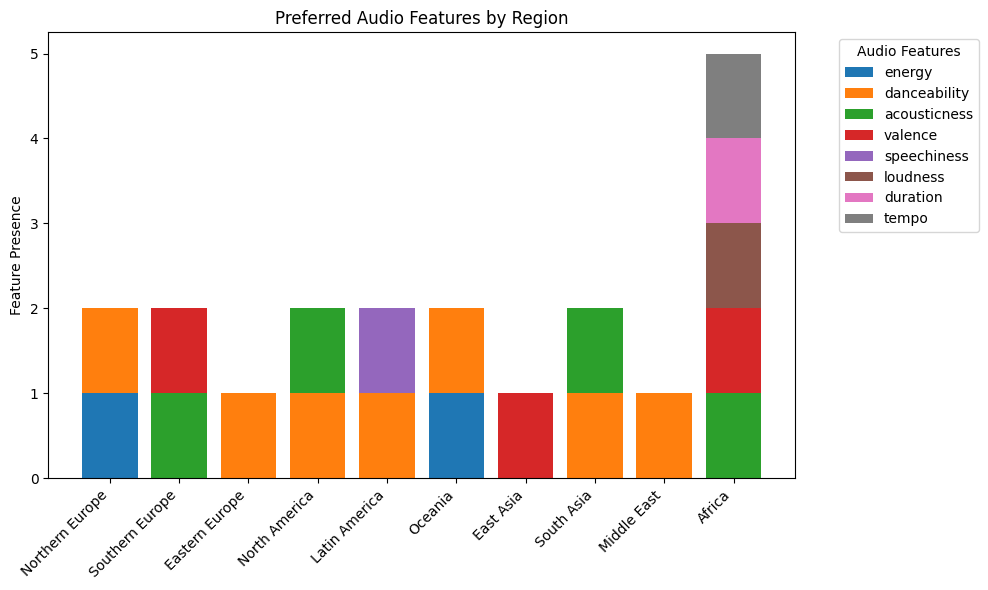
\includegraphics[width=\textwidth]{media/feature_preferences_regions.png}  
        \caption{Regional preferences}
    \end{minipage}
\end{figure}

